\documentclass[12pt]{article}
\usepackage[utf8]{inputenc}
\usepackage{float}
\usepackage{amsmath}
\usepackage{amssymb}
\usepackage{multicol}
\usepackage{tikz}
\usepackage[shortlabels]{enumitem}


\usepackage[hmargin=3cm,vmargin=6.0cm]{geometry}
%\topmargin=0cm
\topmargin=-2cm
\addtolength{\textheight}{6.5cm}
\addtolength{\textwidth}{2.0cm}
%\setlength{\leftmargin}{-5cm}
\setlength{\oddsidemargin}{0.0cm}
\setlength{\evensidemargin}{0.0cm}

%misc libraries goes here

\begin{document}

\section*{Student Information }
%Write your full name and id number between the colon and newline
%Put one empty space character after colon and before newline
Full Name : Berk Ulutaş \\
Id Number :  2522084 \\

% Write your answers below the section tags
\section*{Answer 1}
\subsection*{1)} 
\begin{itemize}
    \item All states are reachable so no need to remove a state.
    \item Initially equivalence classes of $\equiv_0$ are: (namely $K - F$ and $F$) $$\{q_0,q_1,q_3,q_4\} \text{  } \{q_2,q_5\}$$
    \item 
        \begin{tabular}{c|c c}
             & $a$ & $b$\\
            \hline
            $q_0$ & $q_1$ & $q_2$ \\
            $q_1$ & $q_1$ & $q_2$ \\
            $q_3$ & $q_4$ & $q_5 $\\
            $q_4$ & $q_0$ & $q_2$
        \end{tabular}

        \begin{tabular}{c|c c}
             & $a$ & $b$\\
            \hline
            $q_2$ & $q_2$ & $q_3$ \\
            $q_5$ & $q_2$ & $q_3$ 
        \end{tabular}
    \item $\delta (q_0,a) \equiv_0 \delta (q_1,a) \equiv_0 \delta (q_3,a) \equiv_0 \delta (q_4,a)$ and $\delta (q_0,b) \equiv_0 \delta (q_1,b) \equiv_0 \delta (q_3,b) \equiv_0 \delta (q_4,b)$
    \item $\delta (q_2,a) \equiv_0 \delta (q_5,a)$ and $\delta (q_2,b) \equiv_0 \delta (q_5,b)$
    \item After first iteration the classes of $\equiv_1$ are $$\{q_0,q_1,q_3,q_4\} \text{  } \{q_2,q_5\}$$
    \item There is no further splitting of classes, since $\equiv_0$ and $\equiv_1$ classes are same. The algorithm thus terminates.
    \item Minimum-state automaton is: 
    \begin{center}
        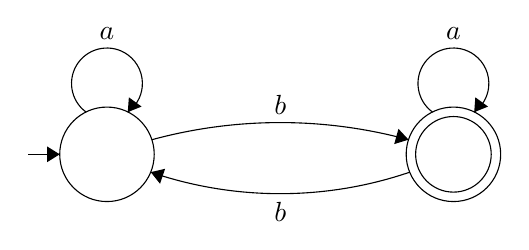
\begin{tikzpicture}[scale=0.2]
            \tikzstyle{every node}+=[inner sep=0pt]
            \draw [black] (20,-24.5) circle (3);
            \draw [black] (42,-24.5) circle (3);
            \draw [black] (42,-24.5) circle (2.4);
            \draw [black] (15,-24.5) -- (17,-24.5);
            \fill [black] (17,-24.5) -- (16.2,-24) -- (16.2,-25);
            \draw [black] (18.677,-21.82) arc (234:-54:2.25);
            \draw (20,-17.25) node [above] {$a$};
            \fill [black] (21.32,-21.82) -- (22.2,-21.47) -- (21.39,-20.88);
            \draw [black] (22.852,-23.573) arc (105.23038:74.76962:31.016);
            \fill [black] (39.15,-23.57) -- (38.51,-22.88) -- (38.24,-23.85);
            \draw (31,-21.98) node [above] {$b$};
            \draw [black] (39.225,-25.634) arc (-71.14392:-108.85608:25.448);
            \fill [black] (22.78,-25.63) -- (23.37,-26.37) -- (23.69,-25.42);
            \draw (31,-27.5) node [below] {$b$};
            \draw [black] (40.677,-21.82) arc (234:-54:2.25);
            \draw (42,-17.25) node [above] {$a$};
            \fill [black] (43.32,-21.82) -- (44.2,-21.47) -- (43.39,-20.88);
        \end{tikzpicture}
    \end{center}
\end{itemize}
\subsection*{2)} 
There is 2 equivalence classes since there is 2 state in minimum-state automaton. Automaton recognizes languages which has odd number of $b$'s. Let $L$ to denote all strings recognized by the automaton. $L = (a^*+ba^*b)ba^*$. Equivalence are: 
\begin{itemize}
    \item $[b] = L$
    \item $[e] = Lba^*$
\end{itemize}
\subsection*{3)} 
According to Myhill-Nerode theorem a language is regular if and only if it has finitely many equivalence classes. To prove $L'$ is not regular we need to show that $L'$ has infinitely many equivalence classes.
\begin{itemize}
    \item Let $S = \{a^nb^m | n,m \in N\}$. $S$ is infinite since it contains one string for each natural number pair $(n,m)$.
    \item Consider any two strings $a^{n_1}b^{m_1} , a^{n_2}b^{m_2} \in S $. Where $n_1 + m_1 \neq n_2 + m_2$
    \item Let $n_1 + m_1 = k_1 + 2u_1$ ($k_1, u_1 \in N$)
    \item Then $a^{n_1}b^{m_1}c^{k_1}d^{u_1} \in L'$ and $a^{n_2}b^{m_2}c^{k_1}d^{u_1} \notin L'$
    \item So $a^{n_1}b^{m_1}$ and $a^{n_2}b^{m_2}$ are distinguishable relative to $L'$. They should be in different equivalence class. 
    \item Since $S$ is infinite we can choose infinitely many such pairs. This means $L'$ has infinitely many equivalence classes. Therefore, by Myhill-Nerode theorem, $L'$ is not regular 
\end{itemize}


\section*{Answer 2}
\subsection*{1)} 
$G = (V, \Sigma, R, S)$ where; \\ 
$V = \{a,b,S,S_1\}$ \\ 
$\Sigma = \{a,b\}$
\begin{equation*}
    \begin{split}
        R = \{S &\rightarrow S_1bS_1, \\ 
        S_1 &\rightarrow aS_1b \text{ } | \text{ }  bS_1a \text{ } | \text{ } S_1S_1 \text{ } | \text{ } bS_1 \text{ } | \text{ } \epsilon \}
    \end{split}
\end{equation*}

\subsection*{2)}
$G = (V, \Sigma, R, S)$ where; \\ 
$V = \{0,1,2,S,S_1,S_2\}$ \\ 
$\Sigma = \{0,1,2\}$
\begin{equation*}
    \begin{split}
        R = \{S &\rightarrow S_1 S_2 \text{ } | \text{ } \epsilon, \\ 
        S_1 &\rightarrow 0 S_1 1 \text{ } | \text{ }  e, \\
        S_2 &\rightarrow 1 S_2 2 \text{ } | \text{ }  e \}
    \end{split}
\end{equation*}
\subsection*{3)}
$G = (V, \Sigma, R, S)$ where; \\ 
$V = \{0,1,S,S_1\}$ \\ 
$\Sigma = \{0,1\}$
\begin{equation*}
    \begin{split}
        R = \{S &\rightarrow 0 S_1 \text{ } | \text{ } 1 S_1, \\ 
        S_1 &\rightarrow 00 S_1  \text{ } | \text{ } 01 S_1  \text{ } | \text{ } 10 S_1  \text{ } | \text{ } 11 S_1  \text{ } | \text{ } e \}
    \end{split}
\end{equation*}


\begin{tikzpicture}
  \node {$S$}
    child {node {0}}
    child {node {$S_1$}
      child {node {0}}
      child {node {1}}
      child {node {$S_1$}
        child {node {1}}
        child {node {1}}
        child {node {$S_1$}
            child {node {0}}
            child {node {0}}
            child {node {$S_1$}
                child {node {$\epsilon$}}
            }
        }
      }
    };
\end{tikzpicture}


\section*{Answer 3}
\subsection*{1)}
$$L_1 = \{e\} \cup \{w \in \{0,1\}^*| \text{ $w$ starts and ends with same symbol}\}$$

\subsection*{2)}
$$L_2 = \{w \in \{0,1\}^* | \text{ $w$ has at least two 1's }\}$$

\end{document}


